% Native publication figure. Requires tikz; retain the adjacent offset table.
\begin{figure}[htbp]
  \centering
  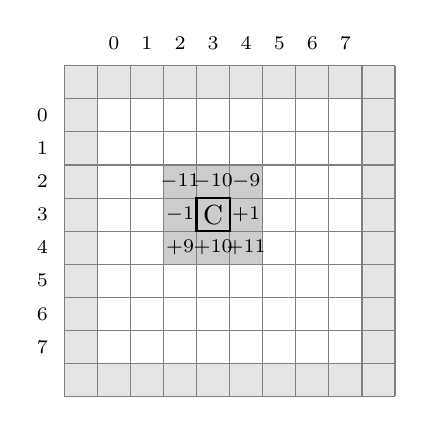
\begin{tikzpicture}[x=0.42cm,y=-0.42cm]
    \fill[black!10] (-0.5,-0.5) rectangle (9.5,9.5);
    \fill[white] (0.5,0.5) rectangle (8.5,8.5);
    \fill[black!20] (2.5,2.5) rectangle (5.5,5.5);
    \foreach \k in {0,...,10} {
        \draw[gray] (\k-0.5,-0.5)--(\k-0.5,9.5);
        \draw[gray] (-0.5,\k-0.5)--(9.5,\k-0.5);
      }
    \draw[thick] (3.5,3.5) rectangle (4.5,4.5);
    \foreach \x/\y/\v in {3/3/-11,4/3/-10,5/3/-9,3/4/-1,5/4/+1,3/5/+9,4/5/+10,5/5/+11}
    \node at (\x,\y) {\scriptsize $\v$};
    \node at (4,4) {C};
    \foreach \k in {0,...,7} {
        \node[above] at (\k+1,-0.7) {\scriptsize\k};
        \node[left] at (-0.7,\k+1) {\scriptsize\k};
      }
  \end{tikzpicture}
  \caption{An eight-by-eight logical board inside a ten-byte-stride allocation. The outer halo remains dead. C is a source cell; the eight labels are relative byte offsets, excluding C itself.}
  \label{fig:life-halo}
\end{figure}
